
\documentclass[letterpaper,hide notes,xcolor={table,svgnames},pdftex,10pt]{beamer}
\def\showexamples{t}


%\usepackage[svgnames]{xcolor}

%% Demo talk
%\documentclass[letterpaper,notes=show]{beamer}

\usecolortheme{crane}
\setbeamertemplate{navigation symbols}{}

\usetheme{MyPittsburgh}
%\usetheme{Frankfurt}

%\usepackage{tipa}

\usepackage{hyperref}
\usepackage{graphicx,xspace}
\usepackage[normalem]{ulem}
\usepackage{multicol}
\usepackage{amsmath,amssymb,amsthm,graphicx,xspace}
\newcommand\SF[1]{$\bigstar$\footnote{SF: #1}}

\usepackage[default]{sourcesanspro}
\usepackage[T1]{fontenc}

\newcounter{tmpnumSlide}
\newcounter{tmpnumNote}

% old question code
%\newcommand\question[1]{{$\bigstar$ \small \onlySlide{2}{#1}}}
% \newcommand\nquestion[1]{\ifdefined \presentationonly \textcircled{?} \fi \note{\par{\Large \textbf{?}} #1}}
% \newcommand\nanswer[1]{\note{\par{\Large \textbf{A}} #1}}


 \newcommand\mnote[1]{%
   \addtocounter{tmpnumSlide}{1}
   \ifdefined\showcues {~\tiny\fbox{\arabic{tmpnumSlide}}}\fi
   \note{\setlength{\parskip}{1ex}\addtocounter{tmpnumNote}{1}\textbf{\Large \arabic{tmpnumNote}:} {#1\par}}}

\newcommand\mmnote[1]{\note{\setlength{\parskip}{1ex}#1\par}}

%\newcommand\mnote[2][]{\ifdefined\handoutwithnotes {~\tiny\fbox{#1}}\fi
% \note{\setlength{\parskip}{1ex}\textbf{\Large #1:} #2\par}}

%\newcommand\mnote[2][]{{\tiny\fbox{#1}} \note{\setlength{\parskip}{1ex}\textbf{\Large #1:} #2\par}}

\newcommand\mquestion[2]{{~\color{red}\fbox{?}}\note{\setlength{\parskip}{1ex}\par{\Large \textbf{?}} #1} \note{\setlength{\parskip}{1ex}\par{\Large \textbf{A}} #2\par}\ifdefined \presentationonly \pause \fi}

\newcommand\blackboard[1]{%
\ifdefined   \showblackboard
  {#1}
  \else {\begin{center} \fbox{\colorbox{blue!30}{%
         \begin{minipage}{.95\linewidth}%
           \hspace{\stretch{1}} Some space intentionally left blank; done at the blackboard.%
         \end{minipage}}}\end{center}}%
         \fi%
}



%\newcommand\q{\tikz \node[thick,color=black,shape=circle]{?};}
%\newcommand\q{\ifdefined \presentationonly \textcircled{?} \fi}

\usepackage{listings}
\lstset{%
  keywordstyle=\bfseries,
  aboveskip=15pt,
  belowskip=15pt,
  captionpos=b,
  identifierstyle=\ttfamily,
  escapeinside={(*@}{@*)},
  stringstyle=\ttfamiliy,
  frame=lines,
  numbers=left, basicstyle=\scriptsize, numberstyle=\tiny, stepnumber=0, numbersep=2pt}

\usepackage{siunitx}
\newcommand\sius[1]{\num[group-separator = {,}]{#1}\si{\micro\second}}
\newcommand\sims[1]{\num[group-separator = {,}]{#1}\si{\milli\second}}
\newcommand\sins[1]{\num[group-separator = {,}]{#1}\si{\nano\second}}
\sisetup{group-separator = {,}, group-digits = true}

%% -------------------- tikz --------------------
\usepackage{tikz}
\usetikzlibrary{positioning}
\usetikzlibrary{arrows,backgrounds,automata,decorations.shapes,decorations.pathmorphing,decorations.markings,decorations.text}

\tikzstyle{place}=[circle,draw=blue!50,fill=blue!20,thick, inner sep=0pt,minimum size=6mm]
\tikzstyle{transition}=[rectangle,draw=black!50,fill=black!20,thick, inner sep=0pt,minimum size=4mm]

\tikzstyle{block}=[rectangle,draw=black, thick, inner sep=5pt]
\tikzstyle{bullet}=[circle,draw=black, fill=black, thin, inner sep=2pt]

\tikzstyle{pre}=[<-,shorten <=1pt,>=stealth',semithick]
\tikzstyle{post}=[->,shorten >=1pt,>=stealth',semithick]
\tikzstyle{bi}=[<->,shorten >=1pt,shorten <=1pt, >=stealth',semithick]

\tikzstyle{mut}=[-,>=stealth',semithick]

\tikzstyle{treereset}=[dashed,->, shorten >=1pt,>=stealth',thin]

\usepackage{ifmtarg}
\usepackage{xifthen}
\makeatletter
% new counter to now which frame it is within the sequence
\newcounter{multiframecounter}
% initialize buffer for previously used frame title
\gdef\lastframetitle{\textit{undefined}}
% new environment for a multi-frame
\newenvironment{multiframe}[1][]{%
\ifthenelse{\isempty{#1}}{%
% if no frame title was set via optional parameter,
% only increase sequence counter by 1
\addtocounter{multiframecounter}{1}%
}{%
% new frame title has been provided, thus
% reset sequence counter to 1 and buffer frame title for later use
\setcounter{multiframecounter}{1}%
\gdef\lastframetitle{#1}%
}%
% start conventional frame environment and
% automatically set frame title followed by sequence counter
\begin{frame}%
\frametitle{\lastframetitle~{\normalfont(\arabic{multiframecounter})}}%
}{%
\end{frame}%
}
\makeatother

\makeatletter
\newdimen\tu@tmpa%
\newdimen\ydiffl%
\newdimen\xdiffl%
\newcommand\ydiff[2]{%
    \coordinate (tmpnamea) at (#1);%
    \coordinate (tmpnameb) at (#2);%
    \pgfextracty{\tu@tmpa}{\pgfpointanchor{tmpnamea}{center}}%
    \pgfextracty{\ydiffl}{\pgfpointanchor{tmpnameb}{center}}%
    \advance\ydiffl by -\tu@tmpa%
}
\newcommand\xdiff[2]{%
    \coordinate (tmpnamea) at (#1);%
    \coordinate (tmpnameb) at (#2);%
    \pgfextractx{\tu@tmpa}{\pgfpointanchor{tmpnamea}{center}}%
    \pgfextractx{\xdiffl}{\pgfpointanchor{tmpnameb}{center}}%
    \advance\xdiffl by -\tu@tmpa%
}
\makeatother
\newcommand{\copyrightbox}[3][r]{%
\begin{tikzpicture}%
\node[inner sep=0pt,minimum size=2em](ciimage){#2};
\usefont{OT1}{phv}{n}{n}\fontsize{4}{4}\selectfont
\ydiff{ciimage.south}{ciimage.north}
\xdiff{ciimage.west}{ciimage.east}
\ifthenelse{\equal{#1}{r}}{%
\node[inner sep=0pt,right=1ex of ciimage.south east,anchor=north west,rotate=90]%
{\raggedleft\color{black!50}\parbox{\the\ydiffl}{\raggedright{}#3}};%
}{%
\ifthenelse{\equal{#1}{l}}{%
\node[inner sep=0pt,right=1ex of ciimage.south west,anchor=south west,rotate=90]%
{\raggedleft\color{black!50}\parbox{\the\ydiffl}{\raggedright{}#3}};%
}{%
\node[inner sep=0pt,below=1ex of ciimage.south west,anchor=north west]%
{\raggedleft\color{black!50}\parbox{\the\xdiffl}{\raggedright{}#3}};%
}
}
\end{tikzpicture}
}


%% --------------------

%\usepackage[excludeor]{everyhook}
%\PushPreHook{par}{\setbox0=\lastbox\llap{MUH}}\box0}

%\vspace*{\stretch{1}

%\setbox0=\lastbox \llap{\textbullet\enskip}\box0}

\setlength{\parskip}{\fill}

\newcommand\noskips{\setlength{\parskip}{1ex}}
\newcommand\doskips{\setlength{\parskip}{\fill}}

\newcommand\xx{\par\vspace*{\stretch{1}}\par}
\newcommand\xxs{\par\vspace*{2ex}\par}
\newcommand\tuple[1]{\langle #1 \rangle}
\newcommand\code[1]{{\sf \footnotesize #1}}
\newcommand\ex[1]{\uline{Example:} \ifdefined \presentationonly \pause \fi
  \ifdefined\showexamples#1\xspace\else{\uline{\hspace*{2cm}}}\fi}

\newcommand\ceil[1]{\lceil #1 \rceil}


\AtBeginSection[]
{
   \begin{frame}
       \frametitle{Outline}
       \tableofcontents[currentsection]
   \end{frame}
}



\pgfdeclarelayer{edgelayer}
\pgfdeclarelayer{nodelayer}
\pgfsetlayers{edgelayer,nodelayer,main}

\tikzstyle{none}=[inner sep=0pt]
\tikzstyle{rn}=[circle,fill=Red,draw=Black,line width=0.8 pt]
\tikzstyle{gn}=[circle,fill=Lime,draw=Black,line width=0.8 pt]
\tikzstyle{yn}=[circle,fill=Yellow,draw=Black,line width=0.8 pt]
\tikzstyle{empty}=[circle,fill=White,draw=Black]
\tikzstyle{bw} = [rectangle, draw, fill=blue!20, 
    text width=4em, text centered, rounded corners, minimum height=2em]
    
    \newcommand{\CcNote}[1]{% longname
	This work is licensed under the \textit{Creative Commons #1 3.0 License}.%
}
\newcommand{\CcImageBy}[1]{%
	\includegraphics[scale=#1]{creative_commons/cc_by_30.pdf}%
}
\newcommand{\CcImageSa}[1]{%
	\includegraphics[scale=#1]{creative_commons/cc_sa_30.pdf}%
}
\newcommand{\CcImageNc}[1]{%
	\includegraphics[scale=#1]{creative_commons/cc_nc_30.pdf}%
}
\newcommand{\CcGroupBySa}[2]{% zoom, gap
	\CcImageBy{#1}\hspace*{#2}\CcImageNc{#1}\hspace*{#2}\CcImageSa{#1}%
}
\newcommand{\CcLongnameByNcSa}{Attribution-NonCommercial-ShareAlike}

\newenvironment{changemargin}[1]{% 
  \begin{list}{}{% 
    \setlength{\topsep}{0pt}% 
    \setlength{\leftmargin}{#1}% 
    \setlength{\rightmargin}{1em}
    \setlength{\listparindent}{\parindent}% 
    \setlength{\itemindent}{\parindent}% 
    \setlength{\parsep}{\parskip}% 
  }% 
  \item[]}{\end{list}} 




\title{Lecture 32 --- Recovery: Repair, Probability }

\author{Jeff Zarnett \\ \small \texttt{jzarnett@uwaterloo.ca}}
\institute{Department of Electrical and Computer Engineering \\
  University of Waterloo}
\date{\today}


\begin{document}

\begin{frame}
  \titlepage

 \end{frame}

\begin{frame}
\frametitle{Probabilistically Answering Queries}

Residues and repairs are not the only way to return consistent answers. 

When there are several options, we can examine these options and make a determination of which is more likely. 

We form candidates - pretenders to the throne of the correct database -  by breaking up the possibilities for repair into all of their possible variants. 

In each candidate database, one tuple from each cluster is selected. 

Both candidate databases will receive a probability of being the ``correct" database.


\end{frame}


\begin{frame}
\frametitle{Remember Salaries?}

\begin{table}[h]\begin{center}
        \begin{tabular}{r | c  c} 
					salaries & employee\_name & salary \\ \hline
	           		 & J. Page  & 50 000 \\ 
	         		 & J. Page  & 80 000 \\ 
					 & V. Smith & 35 000 \\ 
					 & M. Stowe & 75 000 \\ 
        \end{tabular}
\end{center}\end{table}

 In the simplest solution, the database will just answer queries and attach the probability of the answer's correctness as another attribute of the tuple.

\begin{table}[h]\begin{center}
        \begin{tabular}{r | c  c  c} 
					salaries & employee\_name & salary & probability\\ \hline
	           		 & J. Page  & 50 000 & 0.1 \\ 
	         		 & J. Page  & 80 000 & 0.9 \\ 
					 & V. Smith & 35 000 & 0.4 \\ 
					 & M. Stowe & 75 000 & 1 \\ 
        \end{tabular}
\end{center}\end{table}


\end{frame}


\begin{frame}
\frametitle{Are We Sure?}

Suppose the query being asked were all the names of all employees making more than \$70~000. 

In the trivial case, M. Stowe's salary is certainly greater than \$70~000, since its probability is 1 (completely certain). 

Uncertainty enters the picture when examining the J. Page tuples. 

We note probability of his salary being \$80~000 is 0.9, so we include him in the return set and indicate the attached probability.

If the query were names of employees making more than \$45~000, then we would return J. Page with probability 1.

\end{frame}


\begin{frame}
\frametitle{Query Modification}

Or: Modify the requested queries to include the probability attributes. If the original query was:

\texttt{SELECT s.employee\_name FROM salaries s WHERE s.salary > 70~000}


Then the only changes are the addition of\texttt{SUM(s.probability)} and \texttt{GROUP BY s.employee\_name}, so that the rebuilt query reads:


\texttt{SELECT s.employee\_name, SUM(s.probability) FROM salaries s WHERE s.salary $>$ 70~000 GROUP BY s.employee\_name}


\end{frame}


\begin{frame}
\frametitle{The Possibilities Multiply}

In a more complex query, we simply multiply the probabilities. 

\texttt{SELECT o.id, c.id FROM order o, customer c  WHERE o.cIdFk = c.id AND c.balance > 10000 }


This query is modified in the same way as that of the preceding paragraph, except the sum statement reads \texttt{SUM(o.probability * c.probability)}.

The group statement is \texttt{GROUP BY o.id, c.id}.


\end{frame}


\begin{frame}
\frametitle{Determining Probabilities}

The most pressing question is how we determine the probabilities. 

\begin{figure}[!h]
  \centering 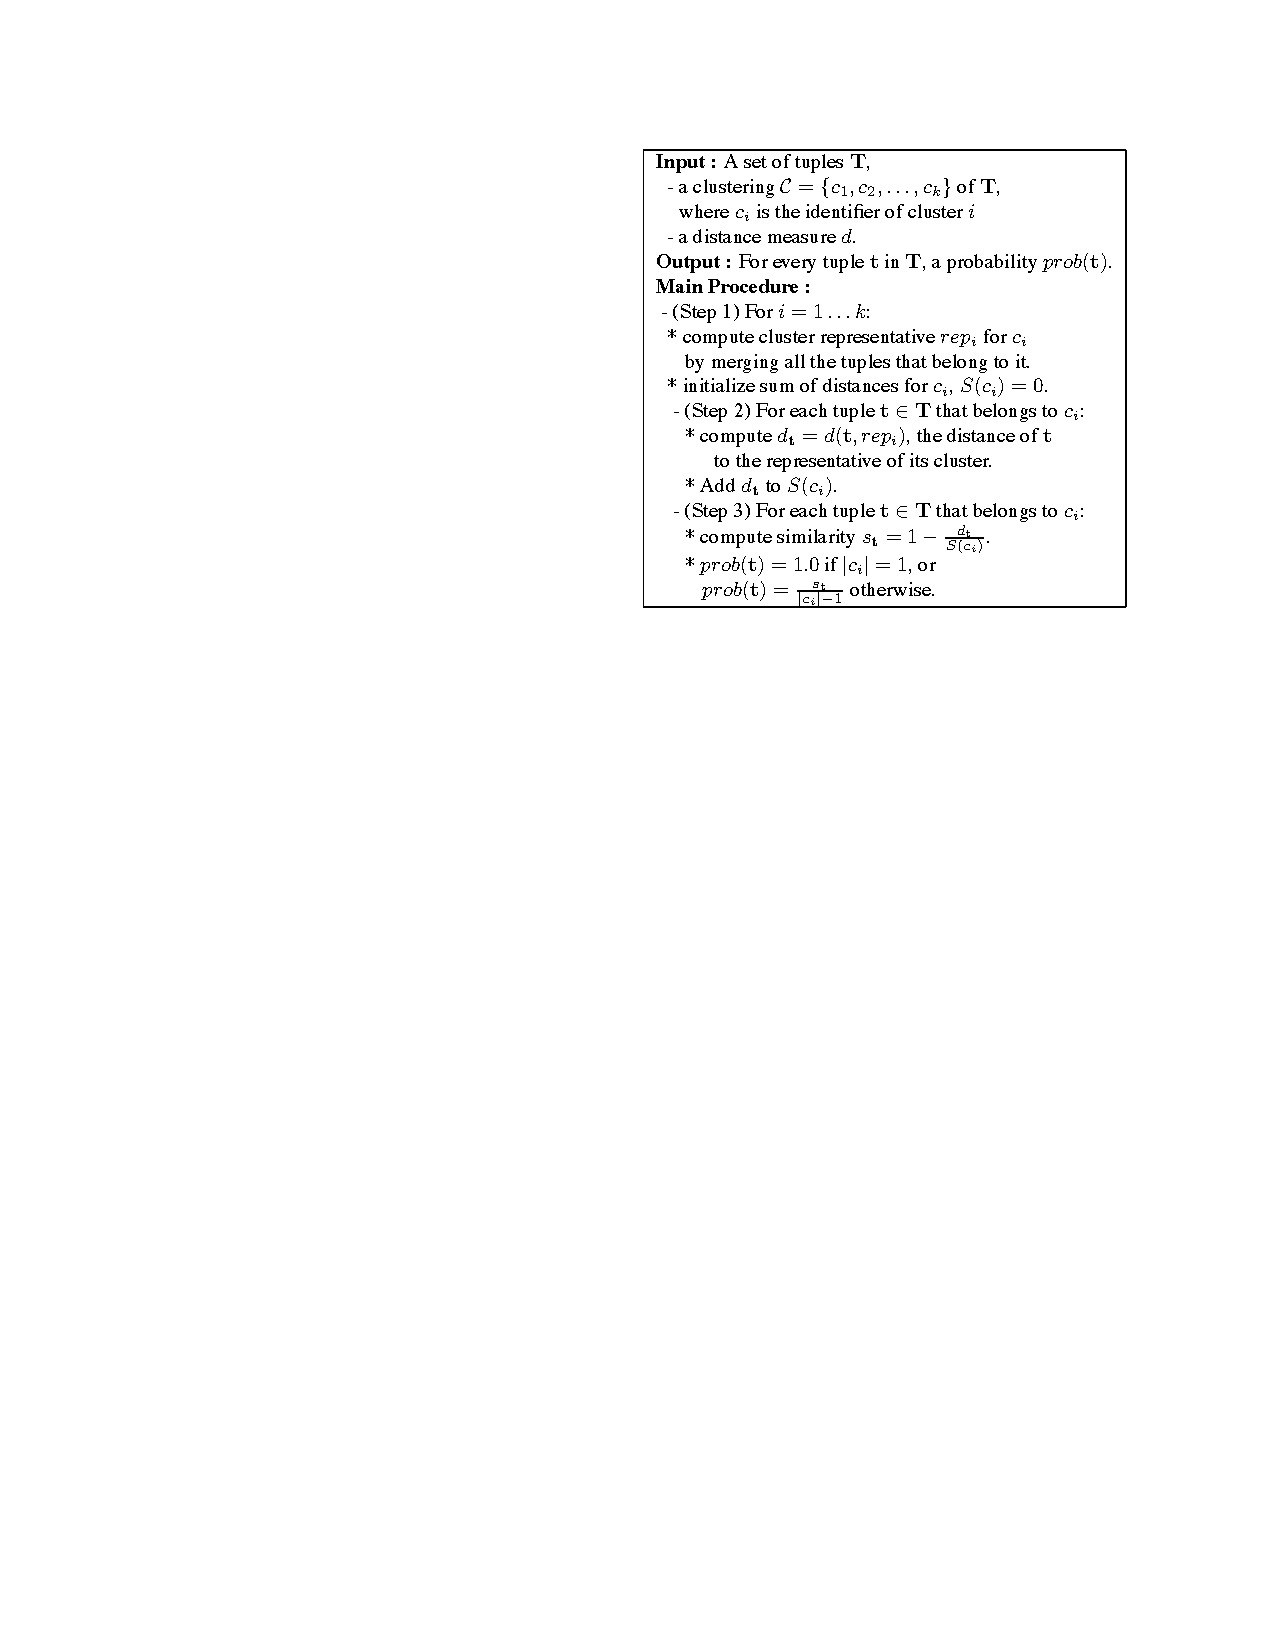
\includegraphics[width=0.6\textwidth]{images/formula.pdf}
\end{figure}

\end{frame}


\begin{frame}
\frametitle{Example: Inconsistent Customers}

\begin{table}[h]\begin{center}
        \begin{tabular}{r | c  c  c  c } 
					customers & name & market\_segment & country & address\\ \hline
	           		 & Mary   & building & USA    & 123 Jones Ave. \\ 
	         		 & Mary   & banking  & Canada & 123 Jones Ave. \\ 
					 & Marion & banking  & USA    & 123 Jones Ave. \\ 
        \end{tabular}
        
\end{center}\end{table}

The most common values in the database are probably the correct ones.

\end{frame}


\begin{frame}
\frametitle{Inconsistent Data Probability}

The algorithm shown above follows this same intuition. 

The tuple we will consider correct is the one closest to the representative. 

For numerical data, similarity between two figures can be computed. 

For data for which there is no obvious distance measure, we term them \alert{categorical data}; information loss as the distance metric.

Information loss is simply a measure of the difference between  the tuple in question and the representative. 

\end{frame}

\begin{frame}
\frametitle{Probabilistically  Imperfect}

The strategy presented is imperfect, however, since we might fail to produce clean answers for some classes of query.

\texttt{select c.id from order o, customer c  where o.quantity < 5 and o.cIdFk = c.id and c.balance > 25~000}. 

This fails because the join between \texttt{c} and \texttt{o} incorrectly double-counts some probabilities.

\end{frame}


\begin{frame}
\frametitle{Choosing the Representative Data?}

Open question: ow we might find a representative sample when it is not obviously in a majority-rules scenario.

Whichever is picked to be the representative will not differ from the representative (by definition), so it will receive a probability of 1. 

Thus, whatever we (perhaps randomly) choose to be our representative is the eventual winner and will be considered correct. 

It is clear that we need to come to some decision, but reporting 100\% certainty about data which is, at best, 50\% certain is misleading. 

\end{frame}

\begin{frame}
\frametitle{Popular Answer...}

This analysis also equates popular with correct.

If an incorrect answer appears in the database twice and a correct answer once, then the incorrect answer will be chosen and deemed correct, since it is more popular. 

That aside, there is not much that can be done about this problem... 

Even a human observing the database might be more likely to conclude that the popular answer is the correct one, in the absence of additional, external knowledge.

\end{frame}


\begin{frame}
\frametitle{Computational Complexity of Repair \& Probability}

Computational complexity is broken down into a short analysis on each of the methods detailed previously.

Computational complexity may disqualify a method from being practically useful, should it take too much time to reach a reasonable answer.



\end{frame}


\begin{frame}
\frametitle{Complexity of Repairs}

Assume that we are looking at repairs that are subsets of the original database.

Then repair checking is in polynomial time for arbitrary constraints combined with acyclic dependencies. 

Should any of these constraints not hold, the problem is pushed into the realm of co-NP-complete problems.


\end{frame}

\begin{frame}
\frametitle{Complexity of Query Transformation}

The process of query transformation is shown to have a polynomial time computability of result tuples. 

The transformed query will be first order as long as the original query is as well. 

The query transformation does not require examining all the possible repairs.

We can evaluate a query with an exponential number of possible repairs in polynomial time.

\end{frame}


\begin{frame}
\frametitle{Aggregate Query Transformation}

Aggregate queries: build a conflict graph; a standard graph with nodes and edges. 

In the graph, maximal independent sets - that is, sets that are the farthest apart in terms of data equality - represent possible repairs of the database. 

As long as there is at most one nontrivial constraint, all operators except \texttt{COUNT} are polynomial time.

If there are many nontrivial constraints, then the problem of finding lower and upper bounds becomes NP-complete. 

The \texttt{COUNT} operation is always NP-complete.


\end{frame}


\begin{frame}
\frametitle{Probabilistic Complexity}

\begin{figure}[!h]
  \centering 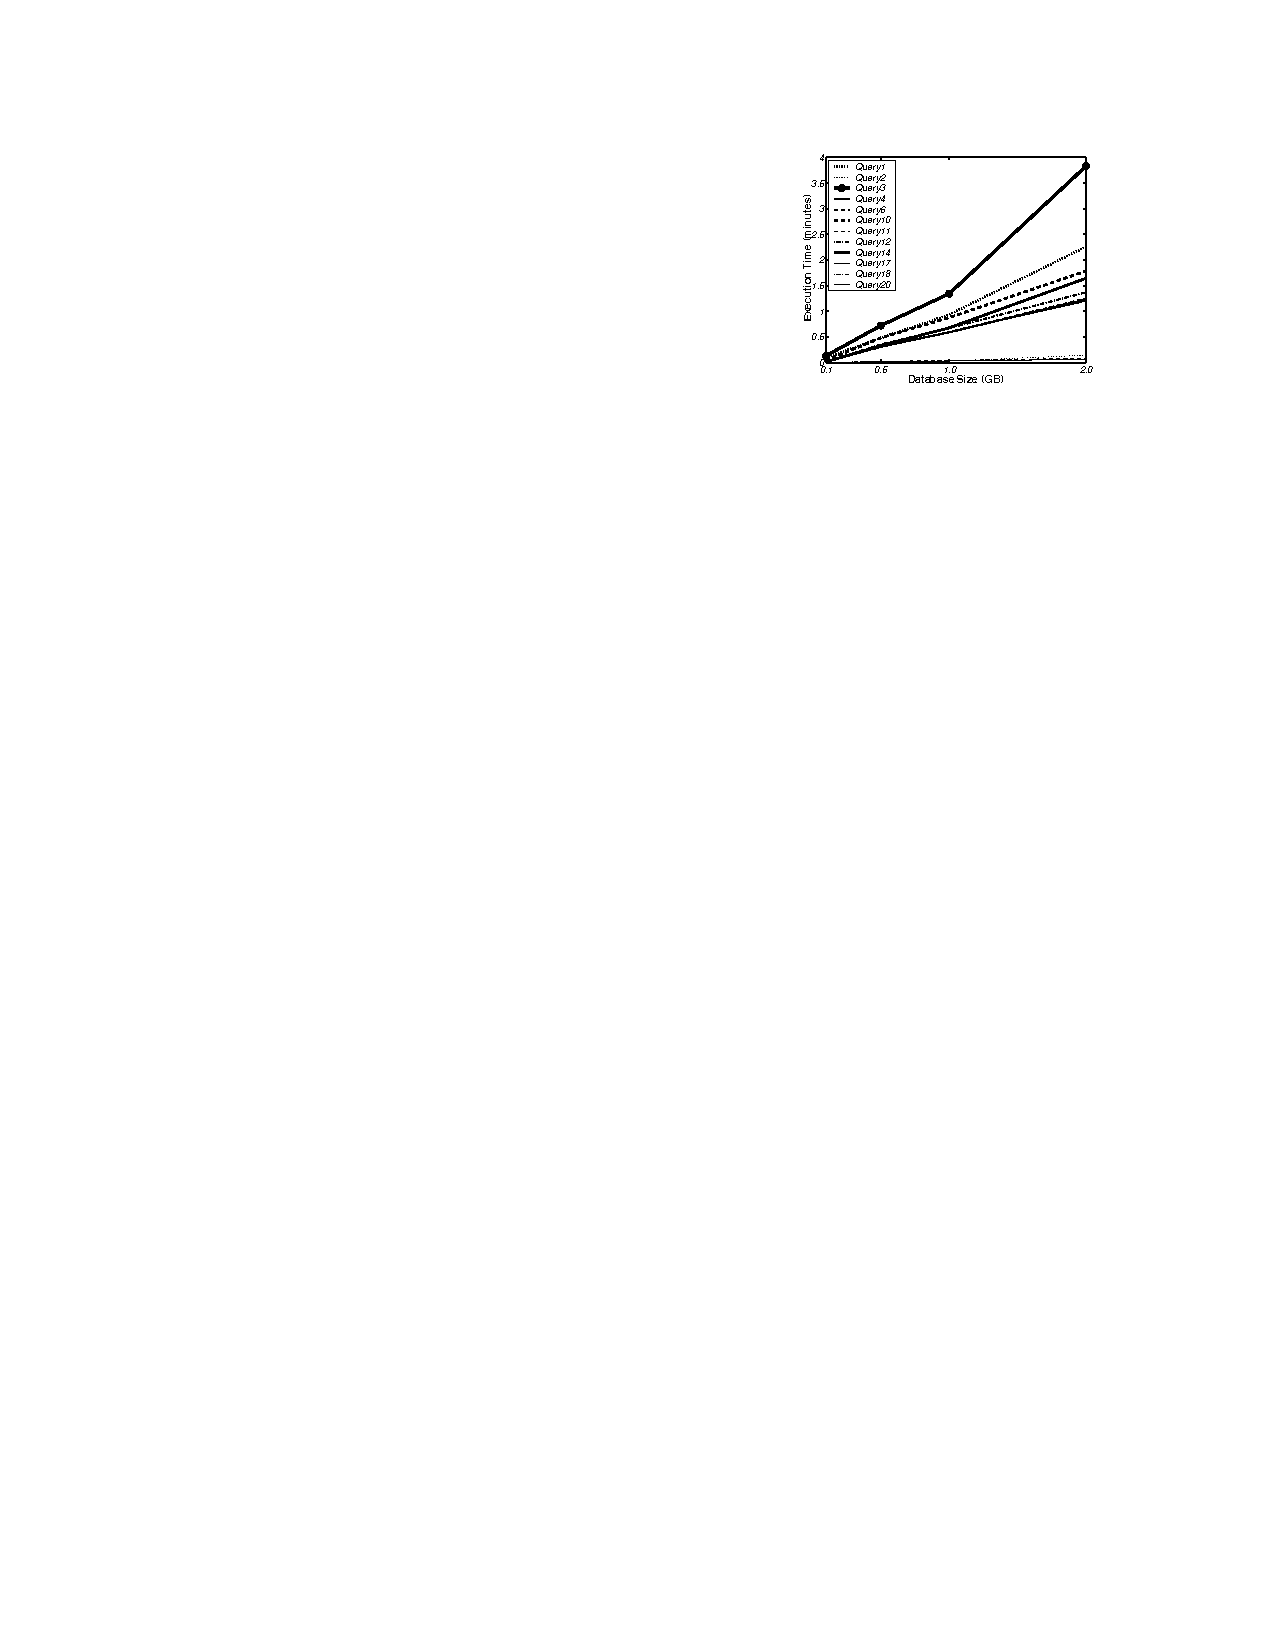
\includegraphics[width=0.8\textwidth]{images/CAPerformance.pdf}
\end{figure}


\end{frame}


\begin{frame}
\frametitle{Future Work}

To get completeness for disjunctive and and existential queries, they will need to move beyond simple query transformations.

Database repairs examined are based on differences against the whole tuple and does not permit modifying attributes of tuples.

The notes cover various deficiencies in the papers that went into this topic...

\end{frame}


\begin{frame}
\frametitle{Conclusion}

There appears to be no single right answer when dealing with an inconsistent database. 

However inconsistent it may be, it is unlikely that we will be able to unequivocally say what is correct and what is not. 

With these techniques, we can certainly get back consistent answers to our queries. 

The success of aggregate queries is less certain, but the chances are still reasonable.


\end{frame}






\end{document}

